%Chapter 7

\renewcommand{\thechapter}{7}

\chapter{Adaptation in Chapel}\label{sec:adaptation_in_chapel}

%\section{Adaptation in Chapel}\label{sec:adaptation_in_chapel}

The goal of this chapter is to present our adaptation in Chapel of the modulo unrolling WU optimization presented in Chapter \ref{sec:transformation}. We also provide a basic understanding of zippered iteration and array slicing, two important features in Chapel used in the optimization's implementation. 

\section{Chapel Zippered Iteration}\label{sec:zippered_iteration}

Iterators are a widely used language feature in the Chapel programming language. Chapel iterators are blocks of code that are similar to functions and methods except that iterators can return multiple values back to the call site with the use of the \textit{yield} keyword instead of \textit{return}. Iterators are commonly used in loops to traverse data structures in a particular fashion. For example, an iterator $fibonacci(n: int)$ might be responsible for yielding the first $n$ Fibonacci numbers. This iterator could then be called in a loop's header to execute iterations 0, 1, 1, 2, 3, and so on. Arrays themselves are iterable in Chapel by default. This is how Chapel can support other important language features such as scalar promotion and whole array assignment. 

Figure \ref{affine_loop}b shows how the original code in Figure \ref{affine_loop}a can be rewritten to use zippered iteration \cite{chamberlain2011user} instead. Zippered iteration is a Chapel language construct that allows multiple iterators of the same size and shape to be iterated through simultaneously. When zippered iteration is used, corresponding iterations are processed together. On each loop iteration, an $n$-tuple is generated, where $n$ is the number of items in the zippering. The $d^{th}$ component of the tuple generated on loop iteration $j$ is the $j^{th}$ item that would be yielded by iterator $d$ in the zippering. 

Zippered iteration can be used with either sequential \textbf{for} loops or parallel \textbf{forall} loops in Chapel. Parallel zippered iteration is implemented in Chapel using leader-follower semantics. That is, a \textit{leader} iterator is responsible for creating tasks and dividing up the work to carry out the parallelism. A \textit{follower} iterator performs the work specified by the leader iterator for each task and generally resembles a serial iterator. 

\section{Chapel Array Slicing}\label{sec:array_slicing}

Chapel supports another useful language feature known as \textit{array slicing}. This feature allows portions of an array to be accessed and modified in a succinct fashion. For example, consider two arrays $A$ and $B$ containing indices from $1..10$. Suppose we wanted to assign elements $A[6]$, $A[7]$, and $A[8]$ to elements $B[1]$, $B[2]$, and $B[3]$ respectively. We could achieve this in one statement by writing $B[1..3] = A[6..8]$. Here, $A[6..8]$ is a slice of the original array $A$, and $B[1..3]$ is a slice of the original array $B$. Line 7 of Figure \ref{affine_loop}b shows examples of two array slices of arrays $A$ and $B$ respectively.

In Chapel, an array slice can support a range of elements with a stride in some cases. For example, in the previous example, we could have made the assignment $B[1..3] = A[1..6$ $by$ $2]$. This would have assigned elements $A[1]$, $A[3]$, and $A[5]$ to elements $B[1]$, $B[2]$, and $B[3]$ respectively. Since all array slices in Chapel are arrays themselves, array slices are also iterable. 

\begin{figure}
\begin{center}
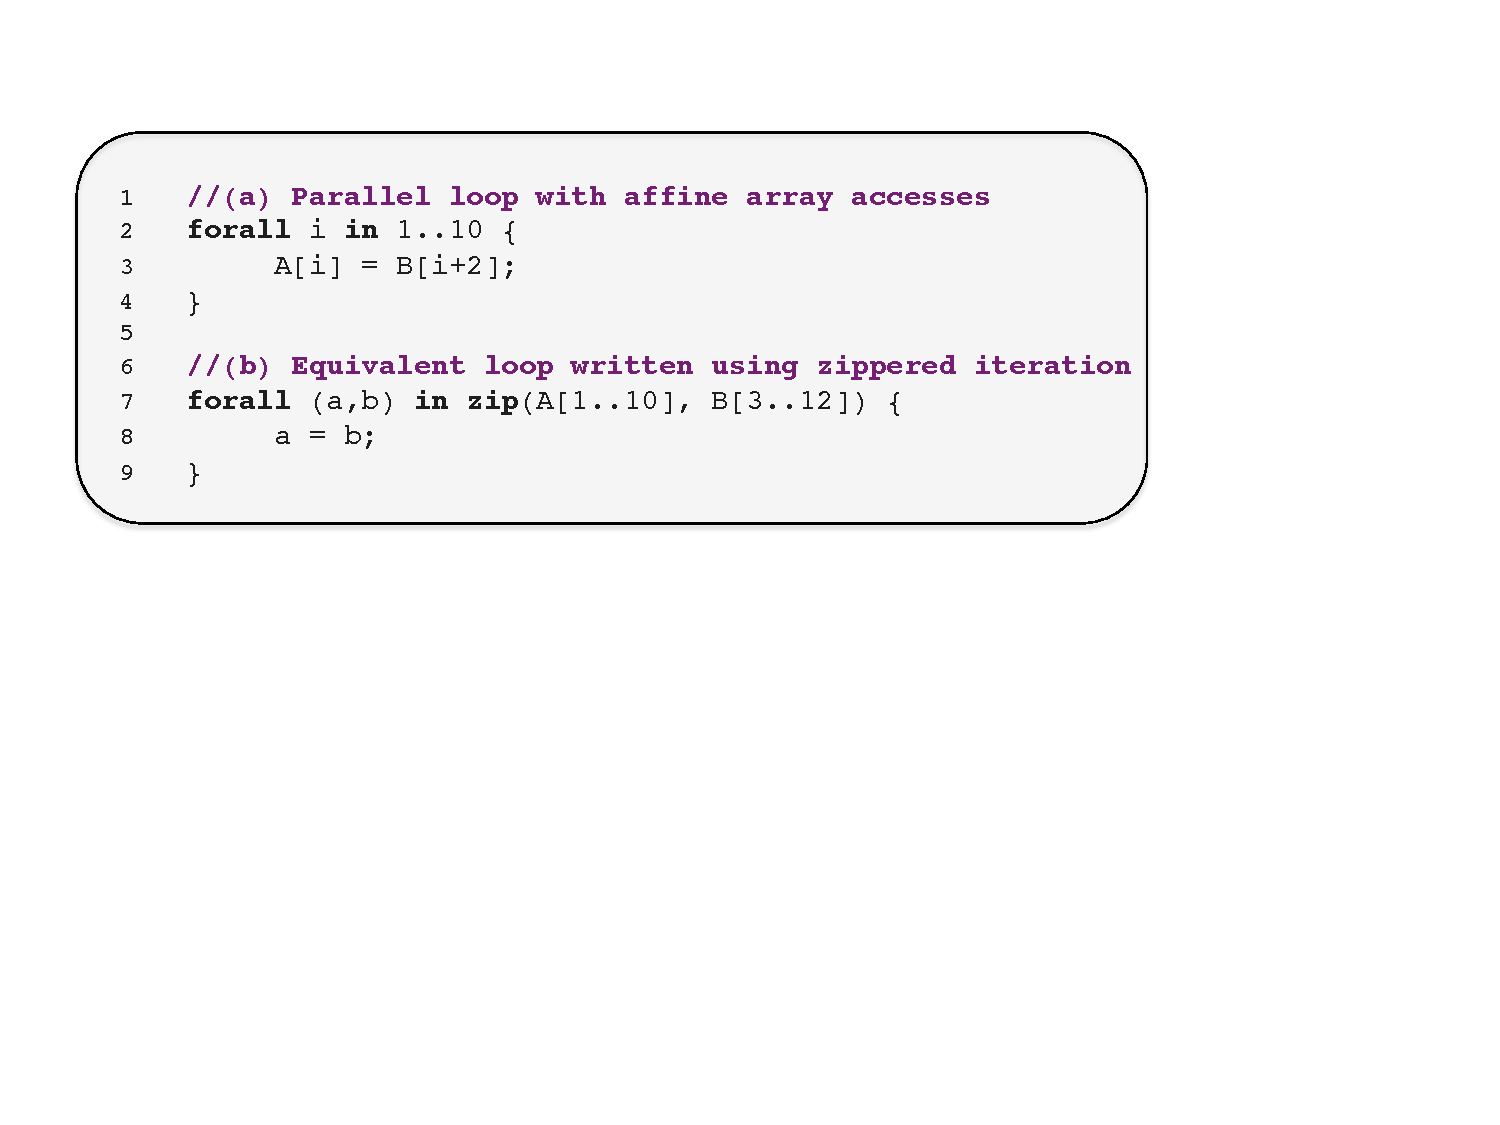
\includegraphics[width=\linewidth]{./Figures/affine_loop}
\renewcommand{\baselinestretch}{1}
\small\normalsize
\begin{quote}
\caption[Chapel parallel affine loop and its equivalent loop written with zippered iterators]{(a) Chapel loop written using a single loop induction variable $i$ ranging from 1 to 10. The loop contains two affine array accesses. (b) The same loop written using zippered iterators in Chapel. Instead of a loop induction variable and a range of values to denote the loop bounds, two array slices each containing the 10 elements accessed by the loop in (a) are specified.\label{affine_loop}}
\end{quote}
\end{center}
\end{figure}

Together, array slicing and parallel zippered iteration can express any parallel affine loop in Chapel that uses affine array accesses. Each affine array access in the loop body is replaced with a corresponding array slice in the loop header, which produces the same elements as the original loop. 

The example code in Figure \ref{affine_loop} shows how regular and zippered iteration versions of the same program have different execution orders but the same result. There are two affine array accesses $A[i]$ and $B[i+2]$ in Figure \ref{affine_loop}a. The loop is written in a standard way where the loop induction variable $i$ takes on values from 1 to 10. Because the loop is a \textbf{forall} loop, loop iterations are not guaranteed to complete in a specific order. This loop assigns elements of array $B$ to $A$ such that the $i^{th}$ element of $A$ is equal to the $(i+2)^{th}$ element of $B$ after the loop finishes. In Figure \ref{affine_loop}b, the same loop is written using zippered iterators. The loop induction variable $i$ no longer needs to be specified, and each affine array access has been replaced with an array slice in the zippering of the loop header. It is possible to transform an affine loop in this fashion even when an affine array access has a constant factor multiplied by the loop induction variable. The resulting array slice will contain a stride equal to the constant factor. The two loops in Figure \ref{affine_loop} are equivalent and generate the same results, but they differ in their execution.

\begin{figure}
\begin{center}
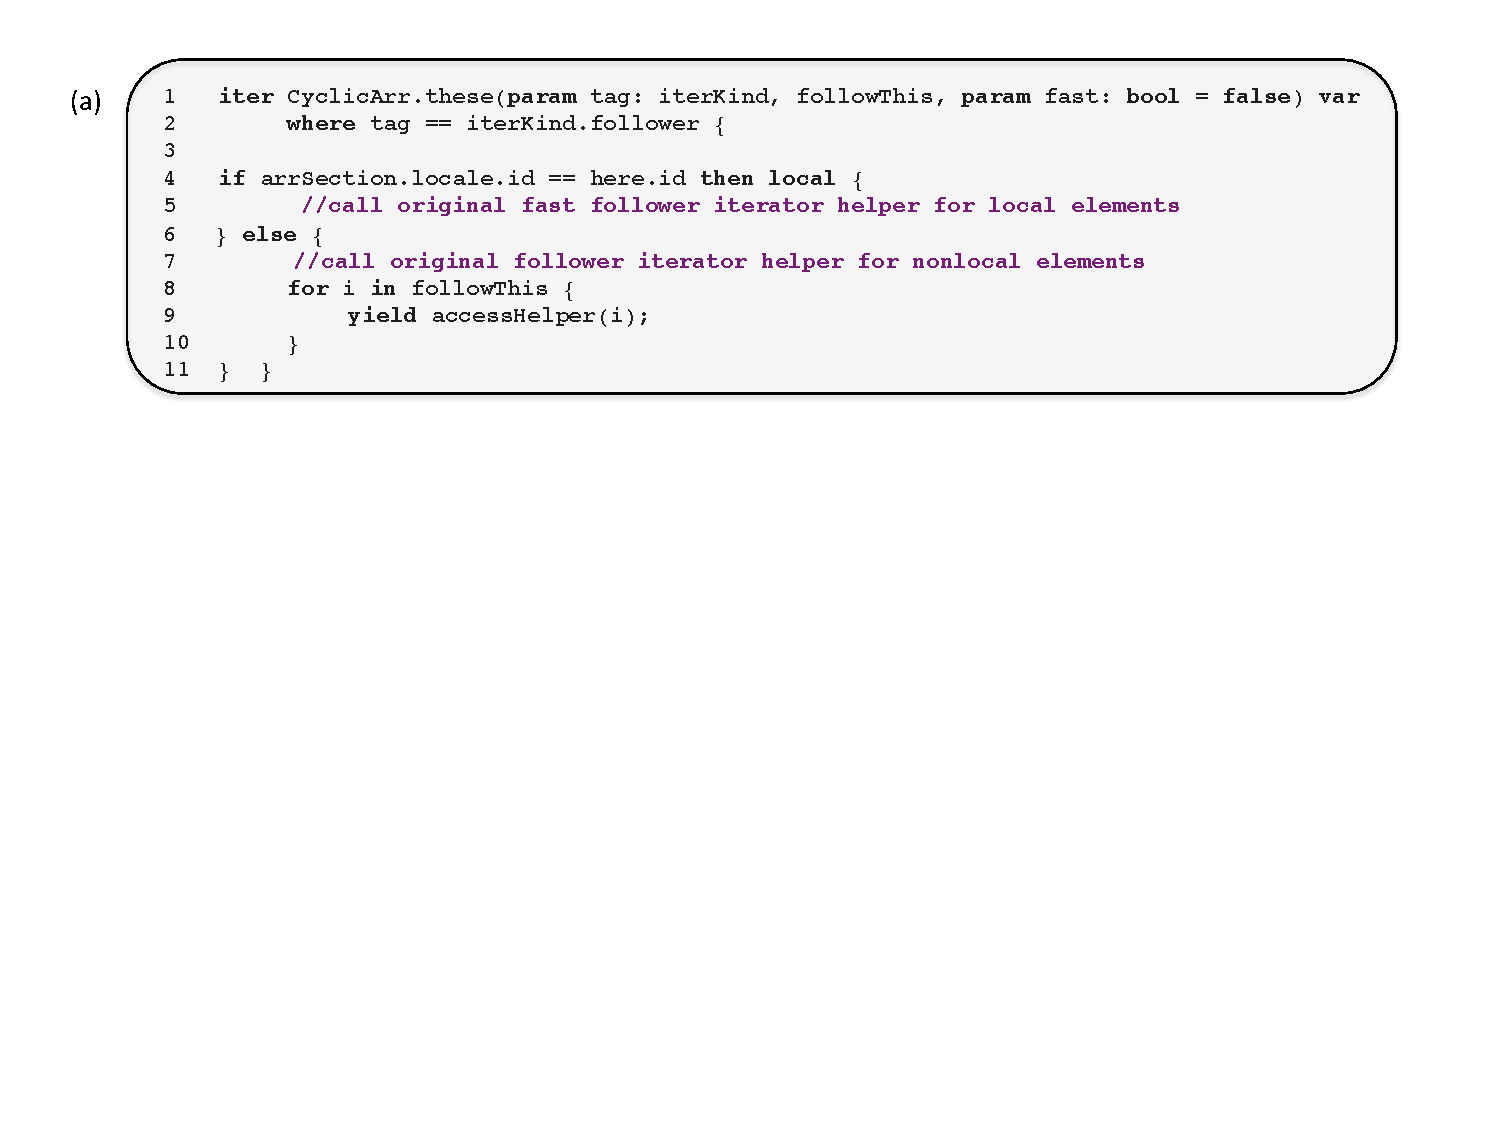
\includegraphics[width=\linewidth]{./Figures/cyclic_muwu_follower_before}
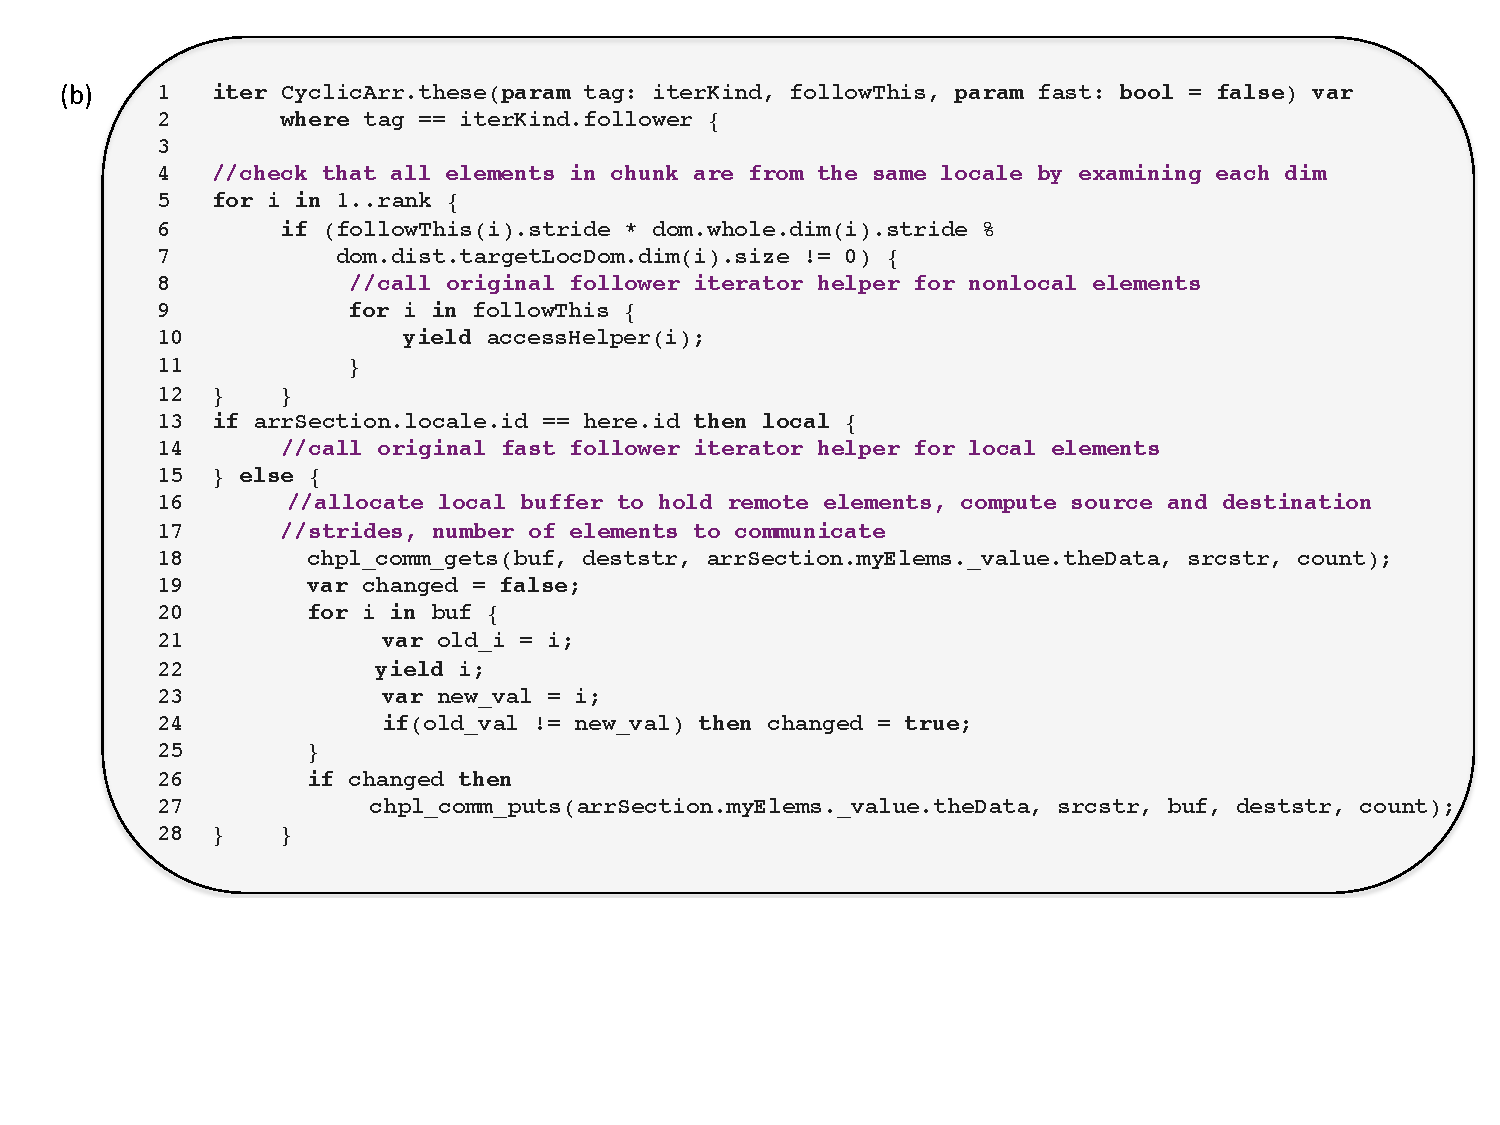
\includegraphics[width=\linewidth]{./Figures/cyclic_muwu_follower_after}
\renewcommand{\baselinestretch}{1}
\small\normalsize
\begin{quote}
\caption[The Chapel Cyclic distribution's follower iterator modified to perform modulo unrolling WU]{(a) Pseudocode for the unaltered Cyclic distribution follower iterator. The code only handles cases when a chunk of work is either completely local or remote. In the remote case in lines 6-11, remote data elements are accessed one at a time, resulting in multiple messages. (b) Pseudocode for the Cyclic distribution follower iterator that has been modified to perform modulo unrolling WU. Now, the code divides the remote case in (a) into two separate cases: remote from a \textit{single} locale and remote from possibly multiple locales. If the chunk of work is remote from a single locale, we can perform message aggregation.\label{cyclic_muwu_follower}}
\end{quote}
\end{center}
\end{figure}

Because any parallel affine loop can be transformed into an equivalent parallel loop that uses zippered iteration, we observe a natural place in the Chapel programming language in which to implement modulo unrolling WU: the leader and follower iterators of the Cyclic and Block Cyclic distribution. The leader iterator divides up the loop's iterations according to the locales they are executed on and passes this work to each follower iterator in the zippering. The follower iterator can then perform the aggregation of remote data elements according to the work that has been passed to it. 

\begin{figure}
\begin{center}
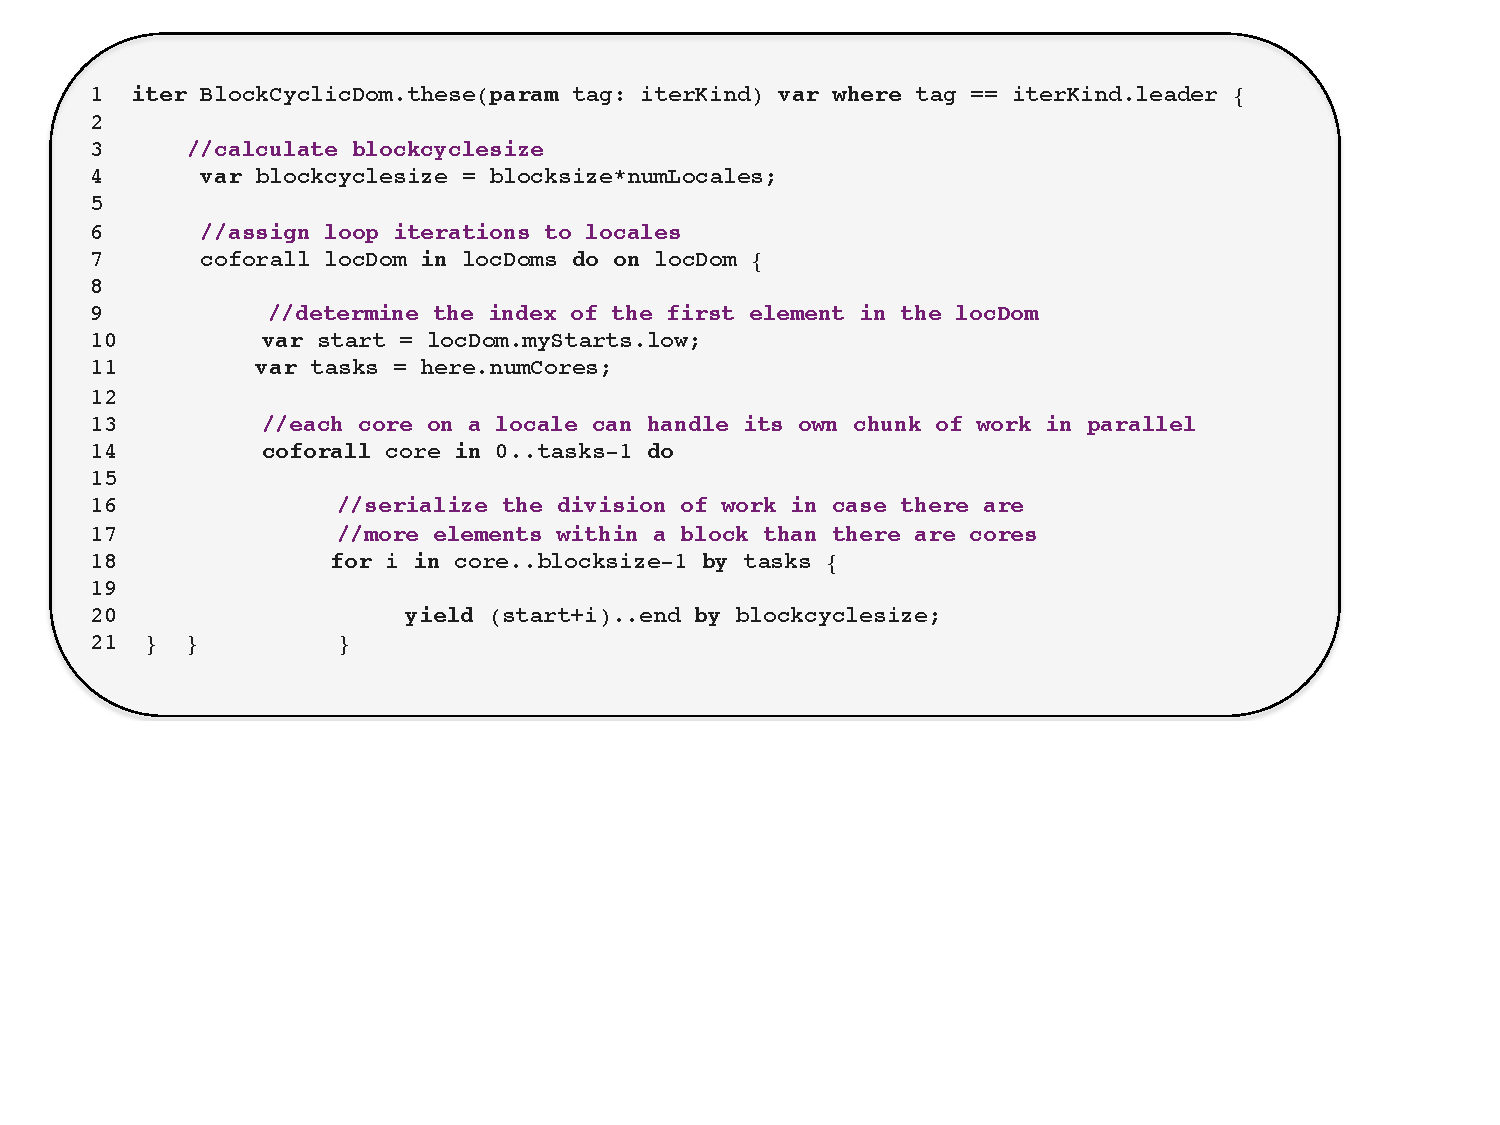
\includegraphics[width=\linewidth]{./Figures/block_cyc_muwu_leader}
\renewcommand{\baselinestretch}{1}
\small\normalsize
\begin{quote}
\caption[The Chapel Block Cyclic distribution's leader iterator modified to perform modulo unrolling WU]{Pseudocode for the Block Cyclic distribution leader iterator that has been modified to perform modulo unrolling WU. Since the leader iterator now splits up the work in a different way than before modification, we do not show the original Block Cyclic leader iterator.\label{block_cyc_muwu_leader}}
\end{quote}
\end{center}
\end{figure}

\section{Implementation}\label{sec:cyclic_modulo}

Modulo unrolling WU is implemented into the Chapel programming language through the Cyclic and Block Cyclic distribution modules, as opposed to being implemented via traditional compiler passes. Specifically, the follower iterator is modified in the Cyclic distribution, and both the leader and follower iterators are modified in the Block Cyclic distribution. Because these modules are written in Chapel, the optimization can be expressed using Chapel's higher-level language constructs, such as zippered iteration and array slicing. 

\begin{comment}
(a) Pseudocode for the unaltered Cyclic distribution follower iterator. The code only handles cases when a chunk of work is either completely local or remote. In the remote case in lines 6-11, remote data elements are accessed one at a time, resulting in multiple messages. (b) Pseudocode for the Cyclic distribution follower iterator that has been modified to perform modulo unrolling WU. Now, the code divides the remote case in (a) into two separate cases. First in lines 5-12, a chunk of work can be remote with elements coming from multiple locales. If so, then data elements are still accessed one at a time like in (a). Second in lines 13-28, a chunk of work can be remote with elements coming from a \textit{single} locale. If so, then it is guaranteed that the elements within the chunk of work are separated by a fixed stride defined by the Cyclic distribution. Therefore, we can aggregate all remote elements in that chunk into a single message.
\end{comment}

Figure \ref{cyclic_muwu_follower} shows the Chapel pseudocode representation of the Cyclic follower iterator before and after it has been modified to perform modulo unrolling WU. Some coding details are left out for brevity. The follower iterator is responsible for carrying out the loop iterations that are passed to it by the leader iterator. Because the follower iterator has no knowledge about how the leader iterator divides up the loop iterations, this chunk of work can fall into one of three cases. It can either be entirely local, entirely remote to a single locale, or spread across multiple locales. In Figure \ref{cyclic_muwu_follower}a, which shows the existing Cyclic follower iterator, the code only handles cases where the chunk of work \textit{followThis} is completely local or remote from possibly multiple locales. If the chunk is local, a helper function responsible for yielding local elements is called on line 5. If the chunk is remote, each remote element is accessed individually with its own message, as shown in lines 6-11. 

Figure \ref{cyclic_muwu_follower}b shows the Cyclic follower iterator modified to perform modulo unrolling WU. Now, all three cases are handled. The first case is when the follower iterator chunk is remote from possibly multiple locales, and it is handled on lines 5-12. If so, then data elements are still accessed one at a time in the way identical to the original follower iterator. The second case, where the follower iterator chunk is completely local, is handled on lines 13-14. Finally, the third case where the chunk of work is remote to a \textit{single} locale is handled on lines 15-28. If so, then it is guaranteed that the elements within the chunk of work are separated by a fixed stride defined by the Cyclic distribution. This stride information is available to access from within the follower iterator. Therefore, we can aggregate all remote elements in that chunk into a single message.

Some details about how the aggregation takes place in the Cyclic follower implementation follow. The entire chunk of work, specified by the \texttt{arrSection} pointer, is communicated to the local \texttt{buf} in one message with the \texttt{chpl\_comm\_gets} call on line 18. Then, elements in this buffer are yielded back to the loop following zippered iteration semantics. The values in \texttt{buf} are compared before and after they are yielded in order to determine whether or not they were written to in the loop body. If so, a \texttt{chpl\_comm\_puts} call on line 27 is required to write all \texttt{buf} elements back to the remote locale.

The implementation of modulo unrolling WU into the Block Cyclic distribution is nearly identical to Figure \ref{cyclic_muwu_follower} with one key addition: the Block Cyclic leader iterator is also altered so that chunks of work that it creates only contain elements that reside in the same position within a block. 
Figure \ref{block_cyc_muwu_leader} shows a Chapel pseudocode representation of the modified Block Cyclic leader iterator, with some coding details left out for brevity. Line 5 computes $blockcyclesize$, the product of the block size parameter and the total number of locales. Lines 8-22 assign loop iterations to locales according to how the leader's caller is distributed. Each object $locDom$ referenced on line 8 represents the collection of ranges of elements of the leader's caller that reside on a single locale. Using this collection, the index of the first element of the first block of the leader's caller, called $start$ is determined, as shown on line 11. Then, the leader iterator determines the offset within each block, denoted by $i$ on line 19. The leader iterator also has knowledge of the total size of its caller, and this is denoted by $end$. Finally, the leader yields a range containing a statically disambiguated portion of its caller. 

Chapter \ref{transformations} described three steps necessary to perform modulo unrolling WU -- (1) block cyclic transformation for static disambiguation; (2) owning expression calculation; and (3) message aggregation. In the next three paragraphs, we discuss how each of those three steps is manifested in the Chapel implementation. 

As stated in Chapter \ref{sec:block_cyclic_transformation}, the \textit{block cyclic transformation to ensure static disambiguation} is not required for the Cyclic distribution because a Cyclic distribution is equivalent to a Block Cyclic distribution with a block size parameter equal to 1, and this transformation is only required for Block Cyclic distributions with block sizes greater than 1. However, we explicitly perform the \textit{block cyclic transformation to ensure static disambiguation} in the Block Cyclic leader iterator. Each range yielded by the Block Cyclic leader in line 21 of Figure \ref{block_cyc_muwu_leader} represents one strip mined portion of the transformed loop in Figrure \ref{transformations}.

Both the Cyclic and Block Cyclic leader iterators already assign loop iterations to locales according to the first item in the zippering by convention, so no \textit{owning expression calculation} is necessary. Choosing to assign iterations based on the first item in the zippering is an accepted convention in the Chapel programming language that cannot be changed without needing to modify the leader iterators of other distributions not explored in this work. The only consequence of not directly implementing the owning expression calculation into the Cyclic and Block Cyclic leader iterators is that the loop will not minimize the number of remote data accesses per iteration. 

Finally, for both the Cyclic and Block Cyclic distributions, the \textit{message aggregation step} takes place in the modified follower iterators. Specifically, lines 15-28 of Figure \ref{cyclic_muwu_follower} directly correspond to lines 3-6 and 14-16 in Figure \ref{transformations}.

We are currently in the process of contributing our source code implementation of modulo unrolling WU to the trunk repository of the Chapel compiler, maintained by Cray Inc. We are working very closely with the researchers at Cray to make this happen. 

\begin{comment}
Modulo unrolling WU is implemented in the follower iterator of the Cyclic distribution. Based on the semantics of parallel zippered iteration, the leader iterator will divide up the iterations of the loop across the locales of the machine according to the first item in the zippering. This could mean that some portions of work will not be local to where the computation is taking place. The follower iterator in the Cyclic distribution recognizes whether or not its chunk of work is local or remote. If remote, all of the remote array elements are brought to the present locale in a local buffer using one \texttt{chpl\_comm\_gets} call. Finally, elements of the local buffer are now yielded back to the loop header. A loop body may modify the elements that are yielded to it via zippered iteration. To account for this, the follower iterator compares the element before it was yielded to the element after it was yielded. If any of the elements in the follower's chunk of work were modified, the entire local buffer is stored back to the remote local via one \texttt{chpl\_comm\_puts} call. 
\end{comment}

%\subsection{Block Cyclic Distribution with Modulo Unrolling WU}\label{subsec:block_cyclic_modulo}

\begin{comment}
For the Chapel Block Cyclic implementation, both the leader and follower iterators have been modified to support the modulo unrolling WU optimization. Modulo unrolling, in its original form, is not compatible with the Block Cyclic distribution because consecutive array elements can reside on the same locale (this is defined by the block size parameter), which destroys the static locality information that we were able to use in the Cyclic distribution. The Block Cyclic leader iterator is now modified to choose slices of work such that the new "stride" is equal to the product of the block size and the cycle size. This way, when the work is passed to the follower iterator, elements that are in the same position within each block are guaranteed to be on the same locale. The follower iterator of the Block Cyclic distribution can now perform modulo unrolling WU in the same way as the Cyclic distribution. 
\end{comment}

